\section{实验与结果}

\subsection{实验设置}

全部实验在一台搭载 NVIDIA GeForce RTX 3060 Laptop GPU（6\,GB）的笔记本电脑上本地运行，操作系统为 Windows~11，软件版本为 Python \VerPython{}、NumPy \VerNumpy{}、scikit-learn \VerSklearn{}、SciPy \VerScipy{}、PyTorch \VerTorch{}、torchvision \VerTorchvision{} 和 OpenCV \VerOpencv{}。39 个试次的特征提取约需三分钟，主要耗时在光流；包括 bootstrap 和置换分析在内的所有模型评估不到两分钟。所有随机步骤使用种子 0。正式运行前，我们先在单个试次（B001）上检查了特征提取器，确认了帧数、5635 个运动学采样点与 5640 帧视频的对齐，以及官方折的成员划分。随后完整流程只运行一次，本报告中的每个数字都读取自其输出文件。

\subsection{定量结果}

表~\ref{tab:main} 和图~\ref{fig:results} 给出了所有模型的结果。多数类基线总是预测新手，在 39 个试次中对 19 个（准确率 \AccMZero{}），macro-F1 为 \FMZero{}，因为中级和专家两类的 F1 都是零。仅运动学基线 K-simple（M1）的 macro-F1 为 \FMOne{}（95\% 区间 \LoMOne{} 至 \HiMOne{}），准确率为 \AccMOne{}。它与多数类的配对差值为 \DOneZero{}，区间 \DLoOneZero{} 至 \DHiOneZero{} 不包含零，精确置换检验给出 $p = \PMOne{}$。因此第一个预先声明的比较得到支持：简单的试次统计量携带可以迁移到新外科医生的技能信息，尽管区间下限接近多数类水平。

\begin{table}[htbp]
\centering
\small
\caption{JIGSAWS 缝合任务上的留一用户结果（39 个试次，8 位外科医生）。Macro-F1、准确率和各类别 F1 均在合并的折外预测上计算。区间为 2000 次用户级 bootstrap 重采样的第 2.5 至 97.5 百分位数；$p$ 为在全部 420 种标签分配上的精确用户级置换检验 $p$ 值。加粗的行分别是运动学基线、主多模态模型和针对性改进。}
\label{tab:main}
\begin{tabular}{@{}l l c c c c c c@{}}
\toprule
模型 & 编号 & Macro-F1 [95\% CI] & 准确率 & F1$_\mathrm{N}$ & F1$_\mathrm{I}$ & F1$_\mathrm{E}$ & $p$ \\
\midrule
\multicolumn{8}{@{}l}{\textit{必做实验}} \\
\quad 多数类 & M0 & 0.218 [0.074, 0.310] & 0.487 & 0.66 & 0.00 & 0.00 & 1.000 \\
\quad K-simple & M1 & \textbf{0.515} [0.272, 0.618] & 0.615 & 0.75 & 0.64 & 0.15 & 0.033 \\
\quad V-appear & M2a & 0.345 [0.125, 0.496] & 0.436 & 0.72 & 0.00 & 0.32 & 0.455 \\
\quad V-dyn & M2b & 0.371 [0.222, 0.467] & 0.487 & 0.75 & 0.36 & 0.00 & 0.348 \\
\quad V-flow & M2c & 0.420 [0.178, 0.576] & 0.513 & 0.67 & 0.59 & 0.00 & 0.240 \\
\quad K-simple + V-dyn, 后期 (主模型) & M3 & \textbf{0.443} [0.247, 0.568] & 0.538 & 0.75 & 0.45 & 0.12 & 0.188 \\
\quad K-simple + V-appear, 后期 & M3b & 0.450 [0.253, 0.567] & 0.538 & 0.72 & 0.50 & 0.13 & 0.133 \\
\quad K-simple + V-flow, 后期 & M3c & 0.481 [0.236, 0.596] & 0.615 & 0.75 & 0.69 & 0.00 & 0.062 \\
\quad K-simple + V-dyn, 早期 & M3d & 0.461 [0.242, 0.564] & 0.615 & 0.74 & 0.64 & 0.00 & 0.036 \\
\addlinespace[2pt]
\multicolumn{8}{@{}l}{\textit{针对性改进}} \\
\quad K-simple + K-texture & M4 & \textbf{0.520} [0.273, 0.619] & 0.615 & 0.75 & 0.67 & 0.14 & 0.074 \\
\quad (K-simple + K-texture) + V-dyn, 后期 & M5 & 0.440 [0.259, 0.526] & 0.538 & 0.73 & 0.45 & 0.13 & 0.157 \\
\addlinespace[2pt]
\multicolumn{8}{@{}l}{\textit{对照实验}} \\
\quad 仅时长 & C1 & 0.375 [0.275, 0.482] & 0.487 & 0.82 & 0.20 & 0.11 & 0.367 \\
\quad K-simple, 对 log 时长残差化 & C2 & 0.342 [0.167, 0.475] & 0.385 & 0.47 & 0.43 & 0.12 & 0.445 \\
\quad K-simple + K-texture, 残差化 & C2t & 0.344 [0.132, 0.509] & 0.385 & 0.38 & 0.53 & 0.12 & 0.371 \\
\bottomrule
\end{tabular}

\end{table}

单独使用时，没有一个视频特征块能与随机水平区分开。V-appear、V-dyn 和 V-flow 的 macro-F1 分别为 \FMTwoA{}、\FMTwoB{} 和 \FMTwoC{}，置换检验 $p$ 值分别为 \PMTwoA{}、\PMTwoB{} 和 \PMTwoC{}。在运动学上加入视频没有带来帮助。主多模态模型（M3，K-simple 与 V-dyn 的后期融合）为 \FMThree{}，与 K-simple 的差值为 \DThreeOne{}（区间 \DLoThreeOne{} 至 \DHiThreeOne{}）。区间包含零，因此在当前样本量下第二个预先声明的比较无法区分；但点估计为负，而且其余所有融合变体也都低于单独的 K-simple：与 V-appear 融合为 \FMThreeB{}，与 V-flow 融合为 \FMThreeC{}，与 V-dyn 早期融合为 \FMThreeD{}（图~\ref{fig:results}b）。针对性改进（M4）加入运动纹理特征块后为 \FMFour{}，与 K-simple 的差值 \DFourOne{}（区间 \DLoFourOne{} 至 \DHiFourOne{}）可以忽略，因此第三个预先声明的比较同样没有得到支持。把改进后的运动学模型与 V-dyn 结合（M5）得到 \FMFive{}，同样低于其运动学部分。

\begin{figure}[htbp]
\centering
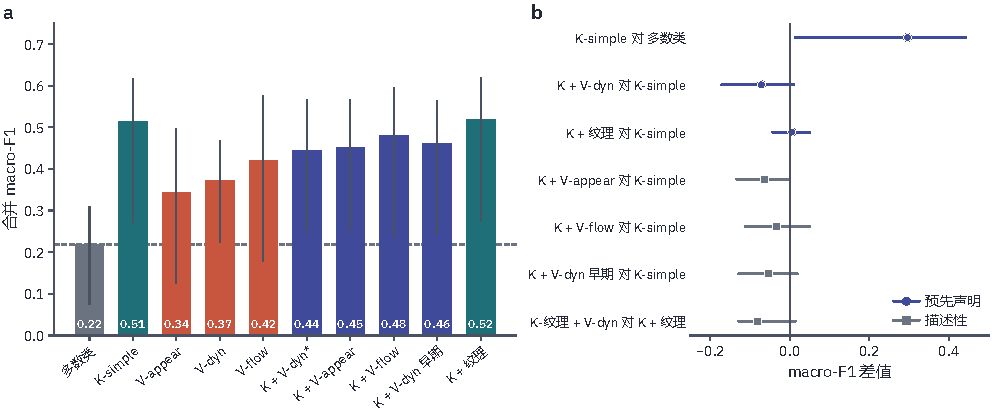
\includegraphics{fig3_results_zh.pdf}
\caption{(a) 多数类、运动学模型（青色）、纯视频模型（红色）和融合模型（蓝色）的合并 macro-F1。误差线为 95\% 用户级 bootstrap 区间；虚线为多数类得分；* 表示预先声明的主多模态模型。(b) macro-F1 的配对差值及其 95\% 用户级 bootstrap 区间。圆点为实验前声明的三个比较，方块为描述性比较。}
\label{fig:results}
\end{figure}

与文献相比，\citet{zia2018rmis} 用近似熵特征在 LOUO 下报告了缝合任务 88.2\% 的准确率。这个数字与我们的结果不能直接比较。在 39 个合并预测下，准确率以 2.56 个百分点为步长变化，88.2\% 不可能出现，所以该文的评估一定使用了不同的试次集合或不同的汇总方式；而且它报告的是准确率而不是 macro-F1。深度网络在 JIGSAWS 上报告的近乎完美的结果大多采用 LOSO，此时测试外科医生也贡献了训练试次\citep{fawaz2018cnn, funke2019video}。我们的 bootstrap 区间在 macro-F1 上宽约 0.25 至 0.4，说明八位外科医生能分辨的差异十分有限\citep{varoquaux2018cv}：只要有一位外科医生的预测类别改变，macro-F1 就可能变化 0.1 以上。

\subsection{成功与失败案例分析}

图~\ref{fig:confusion} 展示了错误出现的位置。三个运动学和多模态模型都能较好地识别新手（K-simple 的 F1 为 \FNMOne{}），对中级的识别中等（F1 \FIMOne{}），但几乎从不识别专家（F1 \FEMOne{}）。在十个专家试次中，K-simple 把五个判为新手、四个判为中级、一个判为专家。图~\ref{fig:users} 按外科医生给出了细分。新手 B、G 和中级 C、F 大多被正确分类（4/5 或 5/5），而专家 D 在每个运动学模型中只有一个试次正确，专家 E 则一个都没有。这种失败有其结构性原因。当一位专家被留出时，训练集中只剩一位专家外科医生，分类器学到的可能是这位外科医生的个人特点，而不是专家的共同之处；身份探针表明这很容易发生：K-simple 仅凭单个试次就能识别外科医生，平衡准确率为 \IdKSimple{}，而随机水平只有 0.125（图~\ref{fig:audit}a）。试次节奏也帮不上忙。专家试次时长的中位数为 \DurE{}\,s，与中级的 \DurI{}\,s 接近，远低于新手的 \DurN{}\,s（图~\ref{fig:data}a），因此时长可以区分新手和受过训练的外科医生，却无法区分两个受训类别。

\begin{figure}[htbp]
\centering
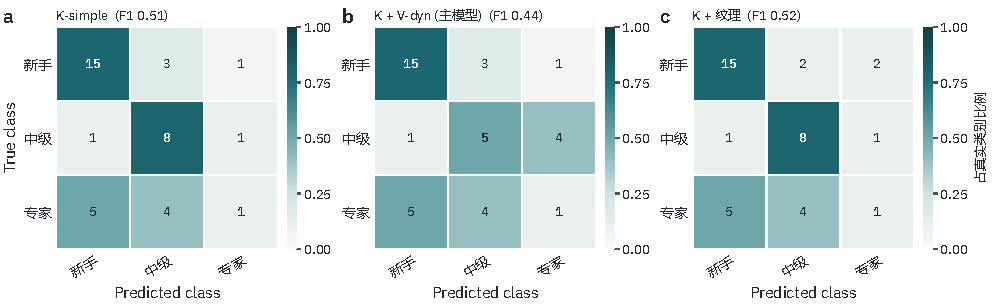
\includegraphics{fig4_confusion_zh.pdf}
\caption{(a) K-simple、(b) 主多模态模型和 (c) 加入运动纹理的 K-simple 的合并混淆矩阵。数字为试次数，颜色表示占真实类别的比例。}
\label{fig:confusion}
\end{figure}

\begin{figure}[htbp]
\centering
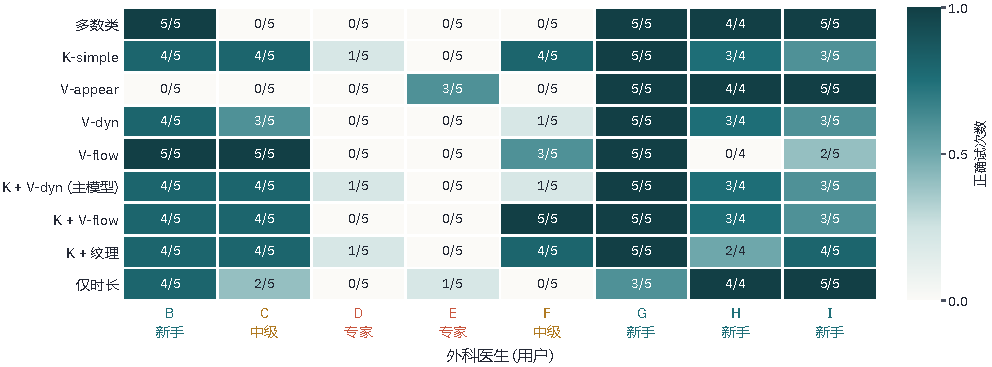
\includegraphics{fig5_users_zh.pdf}
\caption{所选模型在每位被留出外科医生上的正确试次数。每一列是一个 LOUO 折，下方标注该外科医生的技能等级。除 V-appear 外，专家 D 和专家 E 是所有模型的主要失败点；V-appear 则在新手 B 和两位中级外科医生上失败。}
\label{fig:users}
\end{figure}

图~\ref{fig:cases} 在单个试次层面呈现了同样的模式。最明显的成功案例是节奏符合其类别典型水平的试次：新手试次 G001 用时 \CaseGZeroOneDur{}\,s，被判为新手的概率为 \CaseGZeroOnePPred{}；中级试次 C004 用时 \CaseCZeroFourDur{}\,s，被判为中级的概率为 \CaseCZeroFourPPred{}。两位专家则朝相反方向出错，这正是一个学到了“某个人”而不是“某一类”的模型会有的表现。留出 E 时，训练集中唯一的专家是 D，其试次用时 \DurRangeD{}\,s；E 的试次用时 \DurRangeE{}\,s，对专家而言可能显得偏慢，于是五个试次全被判为新手，其中 E001（\CaseEZeroOneDur{}\,s）的新手概率为 \CaseEZeroOnePPred{}，专家概率只有 \CaseEZeroOnePTrue{}。留出 D 时，训练集中唯一的专家是 E，此时训练集里最快的试次属于中级（\DurRangeCF{}\,s），D 的五个试次中有四个被判为中级，包括全数据集最短的试次 D005（\CaseDZeroFiveDur{}\,s），其中级概率为 \CaseDZeroFivePPred{}，专家概率为 \CaseDZeroFivePTrue{}。并非所有错误都能用时长解释。新手 I 的最后两个试次都用时约两分钟，却以很高的置信度被判为中级（I005，\CaseIZeroFiveDur{}\,s，中级概率 \CaseIZeroFivePPred{}），说明模型也会对试次长度以外的 K-simple 特征作出反应。

\begin{figure}[htbp]
\centering
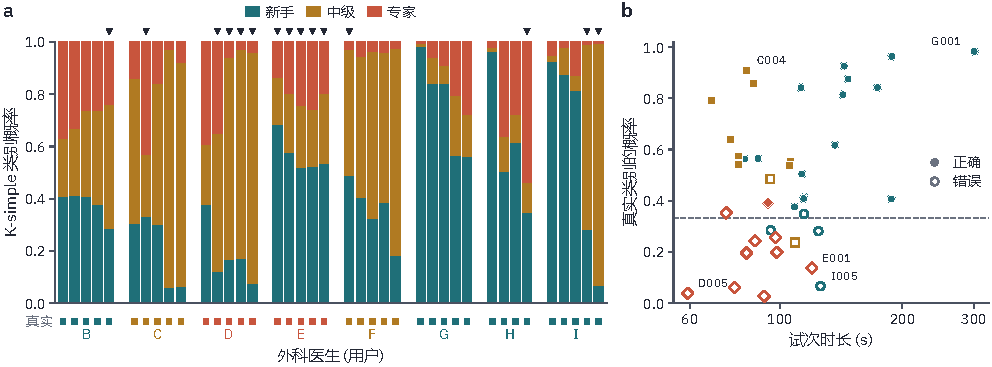
\includegraphics{fig7_cases_zh.pdf}
\caption{K-simple 的试次级预测。(a) 每个试次的类别概率，按被留出的外科医生分组；柱下方块表示真实类别，三角标出预测错误的试次。(b) 真实类别的概率与试次时长（对数坐标）的关系；实心标记为预测正确，空心标记为预测错误，虚线为随机水平（1/3）。图中标注的试次在正文中讨论。}
\label{fig:cases}
\end{figure}

节奏审计显示了运动学信号中有多少是速度。仅用时长的分类器（C1）的 macro-F1 为 \FCOne{}，远高于多数类；K-simple 各特征与 log 时长的绝对相关系数中位数为 \PaceKSimple{}。在训练折内把每个 K-simple 特征对 log 时长做残差化后（C2），macro-F1 从 \FMOne{} 降到 \FCTwo{}；加入纹理特征块时也是如此（C2t，\FCTwoT{}）。因此，K-simple 能迁移到新外科医生的技能信息，主要由试次耗时及随之缩放的量承载（图~\ref{fig:audit}b）。在台式模型任务中，受训外科医生更快，用它区分新手与受训者是合理的，但它并不是质量的度量，这也解释了为什么专家类别被漏判。

\begin{figure}[htbp]
\centering
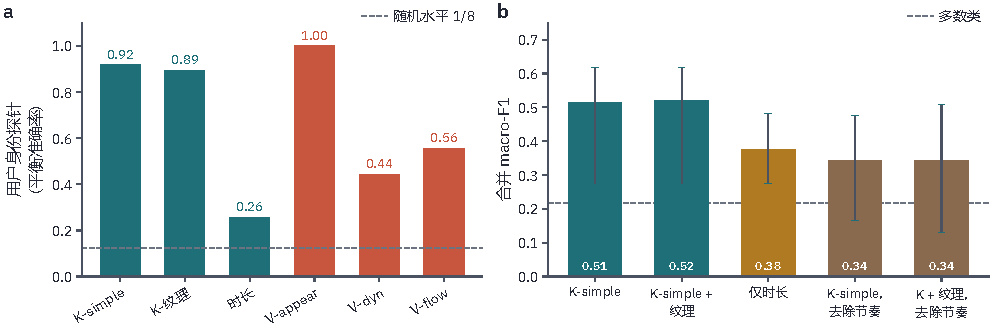
\includegraphics{fig6_audit_zh.pdf}
\caption{捷径审计。(a) 在每个特征块上进行八分类外科医生身份探针的平衡准确率（按试次分层五折），虚线为随机水平。(b) 运动学模型与仅时长分类器、以及在每个训练折内去除与 log 时长线性相关成分后的同一运动学特征的 macro-F1 对比。}
\label{fig:audit}
\end{figure}

视频结果可以用同样两个机制解释。V-appear 能完美识别外科医生（平衡准确率 \IdVAppear{}），但作为技能分类器只有 \FMTwoA{}；图~\ref{fig:users} 呈现出“识别录制场次”的特征模式：新手 G、H、I 的所有试次和专家 E 的三个试次判断正确，而新手 B 和两位中级外科医生的每个试次都判断错误。因此它在专家 E 上的偶然成功不太可能反映技能。V-dyn 的设计目的是抵消静态外观，它携带的身份信息少得多（\IdVDyn{}），却与节奏密切相关：其与 log 时长的绝对相关系数中位数为 \PaceVDyn{}，高于 K-simple。因此它只是提供了运动学模型已有信息的一份更嘈杂的拷贝。在等权重后期融合中，只要视频分类器在运动学判断正确的外科医生上出错，融合结果就会变差。最明显的例子是中级外科医生 F：K-simple 在 5 个试次中对 4 个，V-dyn 只对 1 个，平均之后融合模型只对 \UFMThree{}（图~\ref{fig:users}）。V-flow 在 F 上与运动学互补（融合后 \UFMThreeC{}），但在新手 H 上完全失败，因此其融合结果仍低于单独的运动学模型。

运动纹理改进失败的原因可以从特征本身看出。每个器械的对数无量纲加加速度与 log 时长的相关系数达到 $|r| = \PaceKTextureMax{}$，这与已知的无量纲加加速度对动作时长敏感的结论一致\citep{hogan2009smoothness}；纹理特征块识别外科医生的能力也几乎与 K-simple 相当（\IdKTexture{}）。因此这十个纹理特征在很大程度上重复了 K-simple 已经包含的节奏和身份信息。此外，我们的特征块远小于 \citet{zia2018rmis} 使用的特征集，后者在每个运动学通道上都计算了近似熵；我们没有测试更大的特征集，因为它不在预先声明的协议中，看过这些结果后再去选择它会使比较产生偏差。

\subsection{实现与配置细节}

内层 LOUO 选择在大多数折中选出了较强的正则化（K-simple 在八折中有七折的 $C$ 介于 0.01 与 0.1 之间），这与训练外科医生数量少的情况相符。对 V-appear，内层循环在八折中有六折选择了四个主成分。按照协议，外层折 C、D、E、F 各跳过了一个内层折。K-simple 按外科医生平均的逐折准确率为 \FoldAccMOne{} $\pm$ \FoldSdMOne{}（均值 $\pm$ 标准差），正是这种逐折离散度使我们报告带用户级区间的合并指标，而不是各折的平均值。代码按阶段组织为若干模块（\texttt{data.py}、\texttt{features\_kin.py}、\texttt{features\_video.py}、\texttt{evaluate.py}），\texttt{run\_all.py} 可在约五分钟内从原始数据复现所有模型、预测文件和统计量；\texttt{make\_tables.py} 和 \texttt{make\_figures.py} 可在不重新训练的情况下，从保存的结果重新生成本报告的表格和图。
